% Compile: pdflatex -shell-escape minialu_uvm_intro.tex  (minted requires --shell-escape)
% Packages: texlive-science texlive-latex-extra python3-pygments
\documentclass[aspectratio=169]{beamer}

\usetheme{metropolis}
\usepackage{tikz}
\usetikzlibrary{arrows.meta, positioning, shapes.geometric, fit, backgrounds}
\usepackage{minted}
\usepackage{booktabs}
\usepackage{xcolor}
\usepackage{enumitem}

\title{MiniAlu UVM Verification}
\subtitle{DOOMtang Portfolio --- Step 1}
\author{Isaac G\'omez S\'anchez \\ \small\texttt{github.com/igomsa/DOOMtang}}
\date{}

% ----------------------------------------------------------------
%  Neutral box fill that works regardless of metropolis version
% ----------------------------------------------------------------
\colorlet{boxfill}{gray!12}

\begin{document}

% ============================================================
%  VIDEO 1 --- "What and Why"   slides 1--6
% ============================================================

% ------ Slide 1: Title ----------------------------------------
\begin{frame}
  \titlepage
\end{frame}

% ------ Slide 2: MiniAlu Block Diagram ------------------------
\begin{frame}{MiniAlu: a Tiny Accumulator CPU}
  \begin{center}
  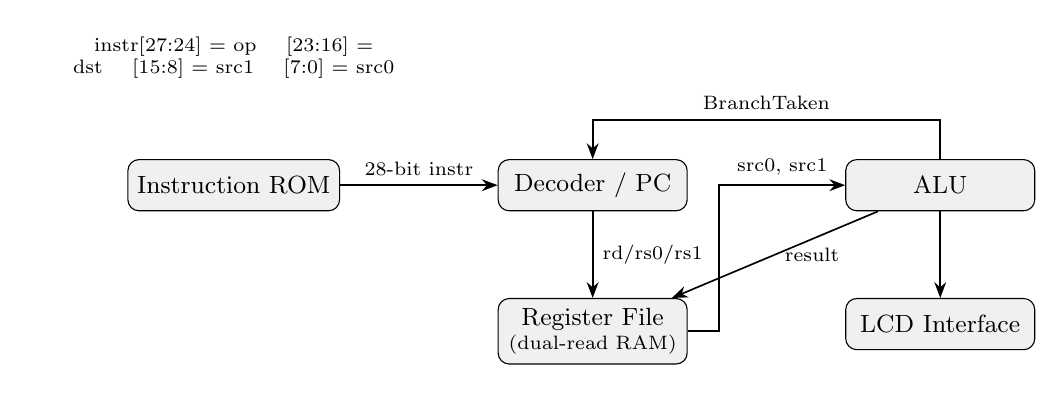
\begin{tikzpicture}[
      box/.style  = {draw, rounded corners,
                     minimum width=2.4cm, minimum height=0.65cm,
                     fill=boxfill, font=\small, align=center},
      arr/.style  = {-Stealth, semithick},
      lbl/.style  = {font=\scriptsize}
    ]

    \node[box]                          (rom)   {Instruction ROM};
    \node[box, right=2cm  of rom]       (decode){Decoder / PC};
    \node[box, below=1.1cm of decode]   (rf)    {Register File\\[-2pt]\scriptsize(dual-read RAM)};
    \node[box, right=2cm  of decode]    (alu)   {ALU};
    \node[box, below=1.1cm of alu]      (lcd)   {LCD Interface};

    \draw[arr] (rom)      -- (decode)  node[midway, above, lbl]{28-bit instr};
    \draw[arr] (decode)   -- (rf)      node[midway, right, lbl]{rd/rs0/rs1};
    \draw[arr] (rf.east)  -- ++(0.4,0) |- (alu.west)
                                       node[near end, above, lbl]{src0, src1};
    \draw[arr] (alu.south) -- (lcd.north);
    \draw[arr] (alu)      -- (rf)      node[midway, right, lbl]{result};
    \draw[arr] (alu.north) -- ++(0, 0.5) -| (decode.north)
                                       node[near start, above, lbl]{BranchTaken};

    \node[above=0.9cm of rom, font=\scriptsize, text width=5cm, align=center]{
      instr[27:24] = op \quad [23:16] = dst \quad [15:8] = src1 \quad [7:0] = src0
    };
  \end{tikzpicture}
  \end{center}

  \vspace{0.2em}
  \begin{columns}
    \column{0.5\textwidth}
      \textbf{Harvard architecture} --- separate instruction ROM and data RAM
    \column{0.5\textwidth}
      8 general-purpose 16-bit registers (\texttt{R0}--\texttt{R7})
  \end{columns}
\end{frame}

% ------ Slide 3: ISA Table ------------------------------------
\begin{frame}{MiniAlu ISA --- 11 Opcodes}
  \begin{center}
  \small
  \begin{tabular}{cll@{\hspace{2em}}l}
    \toprule
    \textbf{Enc} & \textbf{Op} & \textbf{Semantics} & \textbf{} \\
    \midrule
    0  & NOP  & ---                             & \\
    1  & \alert{SUB}  & dst $\leftarrow$ src1 $-$ src0  & \alert{verified in Step 1} \\
    2  & BLE  & branch if src1 $\leq$ src0      & \\
    3  & STO  & dst $\leftarrow$ imm$_{16}$     & load immediate \\
    4  & \alert{ADD}  & dst $\leftarrow$ src1 $+$ src0  & \alert{verified in Step 1} \\
    5  & JMP  & unconditional branch            & \\
    6  & \alert{MUL}  & dst $\leftarrow$ src1 $\times$ src0 (shift-add) & \alert{verified in Step 1} \\
    7  & LCD  & write nibble to LCD             & I/O \\
    8  & \alert{SHL}  & dst $\leftarrow$ src1 \texttt{<<} src0$_{\text{addr}}$ & \alert{verified in Step 1} \\
    9  & CALL & call subroutine                 & saves return addr \\
    10 & RET  & return from subroutine          & \\
    \bottomrule
  \end{tabular}
  \end{center}
  \vspace{0.4em}
  \centering\small Step 1 targets the four \alert{highlighted} computational operations.
\end{frame}

% ------ Slide 4: Verification Problem -------------------------
\begin{frame}{The Verification Problem}
  \begin{alertblock}{Can you spot the bug?}
    \texttt{MUL} in the original RTL uses Verilog's \texttt{*} operator---two
    16-bit signed inputs silently truncated. Is that the intended behavior?
    Overflow? Partial-product semantics? The spec never says.
  \end{alertblock}

  \medskip
  \textbf{Known issues in the \texttt{spartan3E\_tests} codebase:}
  \begin{itemize}
    \item \texttt{<=} (non-blocking) inside \texttt{always @(*)} ---
          sim/synth mismatch, non-deterministic deltas
    \item Blocking \texttt{=} inside clocked \texttt{always @(posedge clk)} ---
          race condition
    \item Duplicate \texttt{case 6:} label in ROM decoder ---
          last branch silently wins
  \end{itemize}

  \medskip
  \textbf{Without a testbench, none of these fire a warning in simulation.}

  \medskip
  \textbf{Goal:} build a UVM environment that \emph{automatically} catches
  any result that disagrees with a golden reference model---including a
  deliberately planted bug.
\end{frame}

% ------ Slide 5: UVM Architecture ----------------------------
\begin{frame}{UVM Environment Architecture}
  \begin{center}
  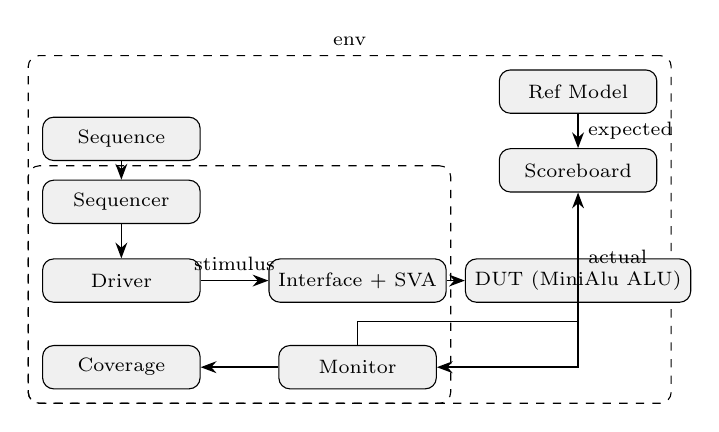
\begin{tikzpicture}[
      box/.style    = {draw, rounded corners,
                       minimum width=2cm, minimum height=0.55cm,
                       fill=boxfill, font=\scriptsize, align=center},
      dashed box/.style = {draw, dashed, rounded corners, inner sep=5pt},
      arr/.style    = {-Stealth, semithick, font=\scriptsize}
    ]

    \node[box] (seq)  at (0.0, 3.2)  {Sequence};
    \node[box] (seqr) at (0.0, 2.4)  {Sequencer};
    \node[box] (drv)  at (0.0, 1.4)  {Driver};
    \node[box] (ifc)  at (3.0, 1.4)  {Interface + SVA};
    \node[box] (dut)  at (5.8, 1.4)  {DUT (MiniAlu ALU)};
    \node[box] (mon)  at (3.0, 0.3)  {Monitor};
    \node[box] (cov)  at (0.0, 0.3)  {Coverage};
    \node[box] (sb)   at (5.8, 2.8)  {Scoreboard};
    \node[box] (ref)  at (5.8, 3.8)  {Ref Model};

    \draw[arr] (seq)  -- (seqr);
    \draw[arr] (seqr) -- (drv);
    \draw[arr] (drv)  -- (ifc)   node[midway, above]{\scriptsize stimulus};
    \draw[arr] (ifc)  -- (dut);
    \draw[arr] (dut.south) |- (mon.east);
    \draw[arr] (mon)  -- (cov);
    \draw[arr] (mon.north) -- ++(0,0.3) -| (sb.south)
                            node[near end, right]{\scriptsize actual};
    \draw[arr] (ref)  -- (sb)    node[midway, right]{\scriptsize expected};

    \begin{scope}[on background layer]
      \node[dashed box, fit=(seqr)(drv)(mon)(cov),
            label={[font=\scriptsize]above left:agent}] {};
      \node[dashed box, fit=(seqr)(drv)(mon)(cov)(sb)(ref),
            label={[font=\scriptsize]above:env}] {};
    \end{scope}
  \end{tikzpicture}
  \end{center}
\end{frame}

% ------ Slide 6: Components in One Line -----------------------
\begin{frame}{UVM Components --- One Line Each}
  \begin{description}[style=nextline, font=\ttfamily\small]
    \item[seq\_item]   Transaction descriptor --- one ALU operation plus expected outputs.
    \item[sequence]    Generates streams of \texttt{seq\_item}s (directed + constrained-random).
    \item[driver]      Applies each item to the DUT through the virtual interface.
    \item[monitor]     Observes DUT outputs; broadcasts to scoreboard and coverage.
    \item[scoreboard]  Calls ref model, compares actual vs.\ expected,
                       calls \texttt{`uvm\_error} on any mismatch.
    \item[coverage]    Bins over opcodes, operand corners, overflow, edge cases.
    \item[env]         Top-level container --- wires agent, scoreboard, coverage together.
    \item[test]        Configures the env and selects which sequence to run.
  \end{description}
\end{frame}

% ============================================================
%  VIDEO 2 --- "How and Demo"   slides 7--11
% ============================================================

% ------ Slide 7: seq_item Snippet ----------------------------
\begin{frame}[fragile]{Sequence Item --- the Transaction}
% TODO: replace snippet with your actual minialu_seq_item.sv once written
\begin{minted}[fontsize=\small, bgcolor=boxfill]{systemverilog}
class minialu_seq_item extends uvm_sequence_item;
  `uvm_object_utils(minialu_seq_item)

  rand logic [3:0]         op;
  rand logic signed [15:0] a, b;
  logic signed [15:0]      result;  // captured from DUT / ref model
  logic                    le;

  constraint valid_op_c {
    op inside {`ADD, `SUB, `MUL, `SHL};
  }
  constraint non_trivial_c {
    !(a == 0 && b == 0);
  }
endclass
\end{minted}
\end{frame}

% ------ Slide 8: Scoreboard / Ref Model -----------------------
\begin{frame}[fragile]{Scoreboard --- Step-and-Compare}
% TODO: replace MUL body with your actual shift-add partial-product tree
\begin{minted}[fontsize=\scriptsize, bgcolor=boxfill]{systemverilog}
function automatic void ref_model(
    input  logic [3:0]         op,
    input  logic signed [15:0] a, b,
    output logic signed [15:0] result,
    output logic               le
);
  case (op)
    `ADD: result = a + b;
    `SUB: result = b - a;
    `MUL: result = /* TODO: shift-add partial-product tree */;
    `SHL: result = b << a[3:0];
    default: result = '0;
  endcase
  le = (b <= a);
endfunction
\end{minted}
  \vspace{0.3em}
  \small Any mismatch triggers \texttt{`uvm\_error} with a timestamped, human-readable report.
\end{frame}

% ------ Slide 9: Coverage Bins --------------------------------
\begin{frame}[fragile]{Functional Coverage}
% TODO: update bins to match your actual minialu_coverage.sv once written
\begin{minted}[fontsize=\scriptsize, bgcolor=boxfill]{systemverilog}
covergroup minialu_cg with function sample(minialu_seq_item tr);
  cp_op: coverpoint tr.op {
    bins add = {`ADD};  bins sub = {`SUB};
    bins mul = {`MUL};  bins shl = {`SHL};
  }
  cp_a_zero:   coverpoint (tr.a == 0);
  cp_b_zero:   coverpoint (tr.b == 0);
  cp_neg_a:    coverpoint (tr.a < 0);
  cp_neg_b:    coverpoint (tr.b < 0);
  cp_overflow: coverpoint (tr.result > 16'sh7FFF || tr.result < -16'sh8000);
  cx_op_zero:  cross cp_op, cp_a_zero, cp_b_zero;
endgroup
\end{minted}
  \vspace{0.2em}
  \small Simulation keeps running until \textbf{all bins are hit} --- random tests drive coverage closure.
\end{frame}

% ------ Slide 10: Demo ----------------------------------------
\begin{frame}{Demo --- Scoreboard Catches a Bug}
  \begin{block}{Setup}
    Planted bug: \texttt{SUB} computes \texttt{a\,$-$\,b} instead of
    \texttt{b\,$-$\,a}.\\
    Directed test: \texttt{op=SUB, a=5, b=3}.
    DUT returns \texttt{+2}; ref model expects \texttt{-2}.
  \end{block}

  \vspace{0.6em}
  % -------------------------------------------------------
  % TODO: replace the block below with an actual screenshot
  %       or pasted terminal transcript from EDA Playground
  %       / Questa showing the UVM_ERROR line and the final
  %       coverage summary.
  %       Use \includegraphics[width=\linewidth]{screenshot.png}
  %       or a minted verbatim block.
  % -------------------------------------------------------
  \begin{alertblock}{TODO --- insert simulation screenshot here}
    Run the testbench on EDA Playground (Questa/VCS), capture the terminal
    output showing the \texttt{UVM\_ERROR} firing on the planted bug and the
    passing coverage summary, then paste or include it here.
  \end{alertblock}
\end{frame}

% ------ Slide 11: Roadmap Teaser ------------------------------
\begin{frame}{What's Next --- DOOMtang Roadmap}
  \begin{columns}
    \column{0.03\textwidth}
    \column{0.28\textwidth}
      \textbf{\alert{Step 1 --- done}}\\[0.5em]
      \small
      SV-UVM on MiniAlu\\
      LED demo on Tang~20k\\[0.3em]
      \textit{This video}

    \column{0.06\textwidth}
      \centering\Large$\Rightarrow$

    \column{0.28\textwidth}
      \textbf{Step 2}\\[0.5em]
      \small
      LOAD/STORE + address bus\\
      SD $\cdot$ HyperRAM $\cdot$ HDMI $\cdot$ USB\\
      Full memory hierarchy

    \column{0.06\textwidth}
      \centering\Large$\Rightarrow$

    \column{0.28\textwidth}
      \textbf{Step 3}\\[0.5em]
      \small
      VexRiscv + UVM lockstep\\
      Spike as scoreboard oracle\\[0.3em]
      \textbf{DOOM on Tang~20k}

    \column{0.01\textwidth}
  \end{columns}

  \vspace{1.2em}
  \centering
  \texttt{github.com/igomsa/DOOMtang}\\[0.3em]
  \small Every step ships a repo, a video, and real passing transcripts.
\end{frame}

\end{document}
